\documentclass[11pt]{article}
\usepackage{geometry}                
\geometry{letterpaper}
\usepackage[]{graphicx}
\usepackage{amssymb}
\usepackage{enumitem}
\usepackage{hyperref}
\usepackage{amsmath}
\usepackage{multicol}
\usepackage{braket}
\usepackage{pdfpages}

\begin{document}

\begin{center}
    {\LARGE Python Implementation of Stabilizer Algorithms }
\vspace{2mm}
{\large \\ Patrick Rall, Iskren Vankov - \today}
\end{center}

% useful for multicolumn figures
\newenvironment{Figure}
  {\par\medskip\noindent\minipage{\linewidth}}
  {\endminipage\par\medskip}


\subsection*{Motivation}
\begin{itemize}
    \item Goal: Implement stabilizer algorithms from the appendix in python
    \item Why python and not C++ as originally planned? 
    \begin{itemize}
        \item We have better familiarity with python and its linear algebra library numpy 
        \item Our first implementation should focus on \textit{correctness} rather than efficiency
        \item We can make graphs and plots and design sophisticated tests to ensure that no bugs are present
    \end{itemize}
    \item Once we have a correct implementation we can copy the code to C++, focusing on optimization rather than algorithmic details
\end{itemize}

\subsection*{Progress so far}
\begin{itemize}
    \item Implementation of $q(x)$ (eq. 42) and state vector coefficient extraction (eq. 46) 
    \item Helper functions: update $D,J$ using (eqs. 48, 49), update $Q,D$ using (eqs. 51, 52)
    \item The \textsc{Shrink} routine and \textsc{Shrink*} routine
    \item The \textsc{RandomStabilizerState} function
\end{itemize}

\subsection*{Questions}
\begin{itemize}
    \item Do the distributions below look correct?
    \item What other tests can you think of to ensure that the code is correct?\\ We already check $G\bar G^T = I$ (mod 2).
    \item Mini project idea: Distribution of MPS Schmidt rank $\chi$ for stabilizer states
\end{itemize}

\subsection*{Next steps}
\begin{itemize}
    \item Implement the remaining routines in the appendix
    \item Begin implementing the main quantum circuit simulator
    \item Begin outlining C++ code
\end{itemize}

\begin{figure}[h]
   \centering
    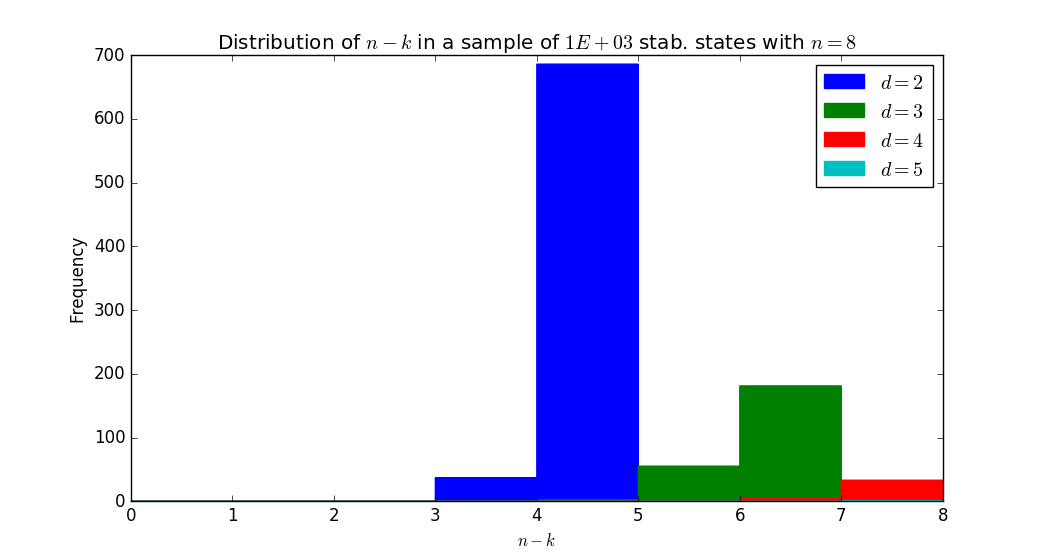
\includegraphics[width=.9\textwidth]{mar14-figs/n-k.png} \\
    \caption{Distribution of sampled $n-k$. In \textsc{RandomStabilizerState}, $d$ is sampled from a probability distribution and $k$ is initially set to $n-d$. Then the \textsc{Shrink*} routine is applied several times, potentially reducing $k$ and increasing $n-k$ a little. Separate colors show the original $d$ values so we can see how many times \textsc{Shrink*} was applied. }
\end{figure}


\begin{figure}[h]
   \centering
    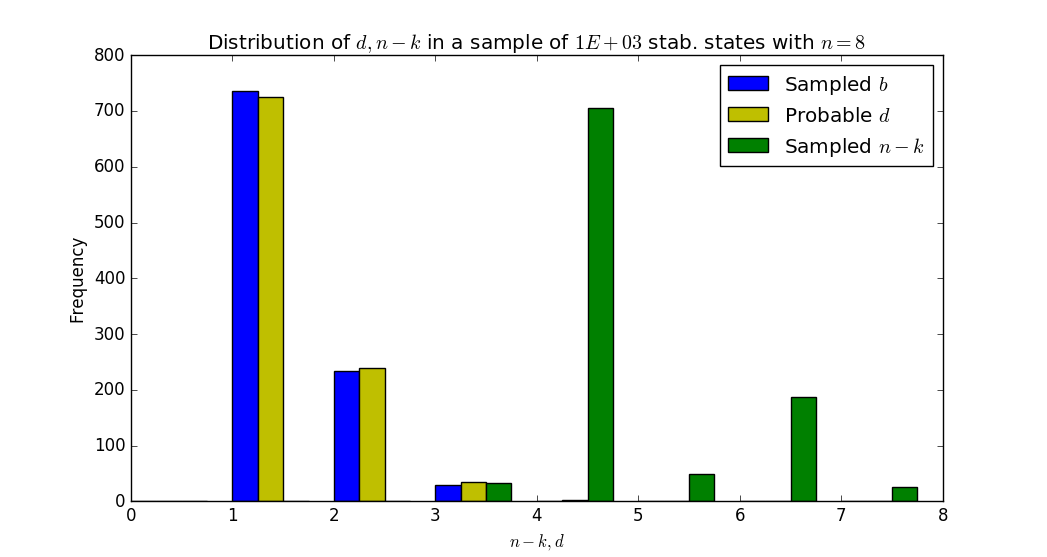
\includegraphics[width=.9\textwidth]{mar14-figs/d_n-k.png} \\
    \caption{Distributions of sampled $b$ and $n-k$, and the scaled probability distribution $P(d)$. We see sampled $d$ and $P(d)$ are very close, but $n-k$ deviates because of the applications of \textsc{Shrink*}. If \textsc{Shrink*} was never applied then the distributions should all be equal.}
\end{figure}



\end{document}

